\section{Lightweight Cryptography}
The term lightweight cryptography refers to cryptographic algorithms that are designed to be secure even when operating in resource-restricted environments. These environments typically have limitations in terms of power, processing capabilities, memory, and even area/space. Lightweight cryptography aims to provide efficient and modernized algorithms that can operate effectively in such constrained settings.



\subsection{The Need for Lightweight Cryptography (LWC)}
Traditional cryptographic algorithms are designed to be secure, but they are often not suitable for environments with limited resources. In recent years, there has been an increasing need for lightweight cryptographic algorithms. This need arises from the growing number of devices connected to the internet. These devices are often small and have limited capabilities.
\newline
The Internet of Things (IoT) refers to a network built by interconnected devices (Figure~\ref{fig:IoT}). These devices gather data from their environment, such as a toaster with a temperature sensor or a sensor in a nuclear power plant, and exchange it with other devices in the network~\cite{chauhan2022analysis}.

\begin{figure}[h]
    \centering
    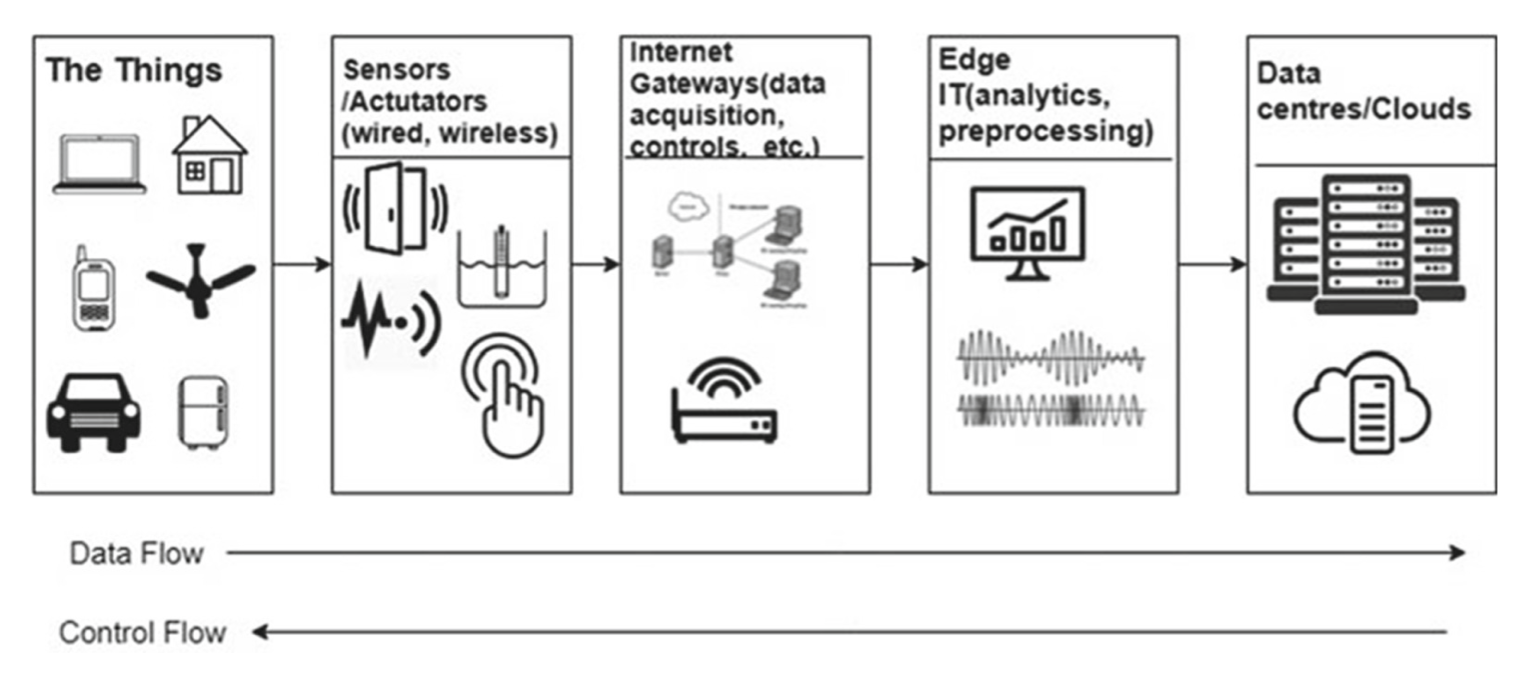
\includegraphics[width=14.0cm, height=6.0cm]{media/DesignofInternetofThings(IoT).png}
    \caption{Design of IoT}
    \label{fig:IoT}
\end{figure}

IoT devices are used in various areas and will become even more important in the future. For example, they are used in:
\begin{itemize}
    \item Smart homes for security monitoring
    \item Smart cities for traffic control and disaster management
    \item Healthcare for patient monitoring
    \item Smart grids for energy management
    \item Self-driving vehicles where cars can generate hundreds of megabytes per second
\end{itemize}
Many of these devices operate in public and sometimes inaccessible areas, making both maintenance and power supply challenging. Additionally, they are often connected over wireless networks, making them vulnerable to node tampering.

\begin{figure}[h]
    \centering
    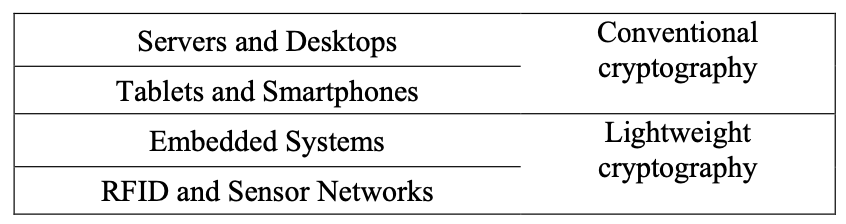
\includegraphics[width=9.0cm, height=2.5cm]{media/device_spectrum.png}
    \caption{Device Spectrum}
    \label{fig:device_spectrum}
\end{figure}

Figure~\ref{fig:device_spectrum} illustrates a rough categorization of devices based on their cryptographic requirements. More specifically, targeted devices can range from microcontrollers with 32-bit down to 4-bit CPUs. In these cases, the narrow data path and limited instruction set of the CPU architecture pose significant constraints. Executing complex cryptographic algorithms on such devices requires many more cycles, further slowing down the process due to potential battery constraints. Additionally, some controllers have as little as 16 bytes of RAM, while RFID devices are even more constrained~\cite{mckay2016report}. Therefore, it is important to have cryptographic algorithms that are secure and do not require excessive resources~\cite{IOTMarkets}~\cite{dhanda2020lightweight}.



\subsubsection{NIST's Endeavor to Standardize LWC}
While the National Institute of Standards and Technology (NIST) has standardized secure algorithms like AES, in the past, these algorithms are not suitable for use in IoT due to the diversity, scalability, and constantly changing nature of these devices~\cite{ekwueme2024lightweight}. However, NIST initiated a project in 2015 to standardize lightweight cryptographic algorithms.

In cryptography, there is always a tradeoff between performance and the required resources to complete a task at every security level.

Understanding the specific security needs of IoT devices is crucial to grasp their requirements. These needs include:

\begin{itemize}
    \setlength{\itemsep}{-5pt}
    \item \textbf{Confidentiality}: Only authorized users or systems should have access to the devices or the network.
    \item \textbf{Availability}: The required data should be available even when multiple simultaneous connections are established.
    \item \textbf{Integrity}: Manipulation of the data should be avoided.
    \item \textbf{Authentication}: Authentication is the process of verifying the identity of a user or device. Due to the diverse range of devices and protocols in IoT networks, achieving authentication and security can be  particularly challenging~\cite{dutta2019lightweight}~\cite{dhanda2020lightweight}.
\end{itemize}

Further, the metrics used to define the requirements for the process of selecting lightweight algorithms are as follows:

\begin{itemize}
    \setlength{\itemsep}{-5pt}
    \item \textbf{Security}: The security of a cipher refers to its ability to resist various types of attacks, including Side Channel Attacks. A minimum key size of at least 128 bits is necessary.
    \item \textbf{Energy consumption}: Many IoT devices run on batteries, thus it is important to minimize power consumption to ensure they can complete their tasks.
    \item \textbf{Latency}: Latency is the time it takes between starting the encryption process and producing the ciphertext. Minimizing latency is crucial for fast-running systems like interconnected cars.
    \item \textbf{Throughput}: Throughput (Kbps) can be thought of as the performance that describes the frequency at which new outputs are generated, which should be in a moderate scale for these devices.
    \item \textbf{Chip Area}: This hardware-specific metric describes the area of a chip implementation measured in gate equivalence (GE) in µm2. The need for area and the consumption of power can be correlated. Consequently, a smaller implementation area can reduce power consumption.
    \item \textbf{Memory Usage}: Efficient memory usage is essential for software applications to ensure optimal performance and resource utilization. Minimizing the amount of memory required for data storage and manipulation can reduce costs and improve scalability~\cite{mckay2016report}.
    \item \textbf{Efficiency}: The ratio between performance and resource demands. Hardware efficiency = Throughput / physical memory, Software Efficiency = Throughput / (Code Size [KB] = algorithm size).
\end{itemize}

\begin{figure}[h]
    \centering
    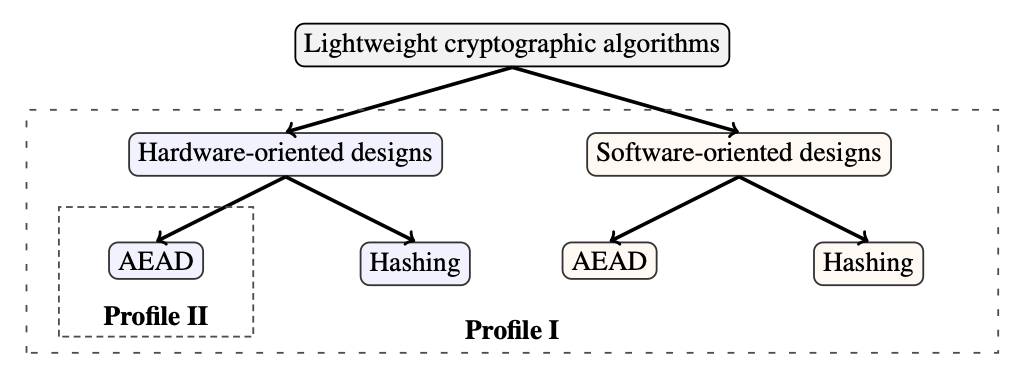
\includegraphics[width=9.0cm, height=3.5cm]{media/profiles.png}
    \caption{Profiles for lightweight cryptography applications}\label{fig:profiles}
\end{figure}

To better understand the needs and define the expectations for lightweight cryptography, NIST conducted a questionnaire among stakeholders. Based on the responses received, NIST created profiles that represent the requirements of these algorithms, which are influenced by the hardware and application areas where these algorithms are needed. The results of this questionnaire led to the creation of two profiles: Profile 1, which focuses on AEAD (Authenticated Encryption with Associated Data) and hashing for constrained software and hardware environments, and Profile 2, which focuses on AEAD for constrained hardware environments Figure~\ref{fig:profiles}. These profiles serve as guidelines for the development and evaluation of lightweight cryptographic algorithms~\cite{mckay2016report}.



\subsection{Security Issues in Lightweight Cryptography}
As mentioned above, IoT devices are openly deployed, processing, and transmitting sensitive and important data, making them high-interest targets for various attacks. Some of these attacks include Denial of Service (DoS) attacks, where the goal is to shut down the targeted system, such as a server, by overwhelming it with a high volume of data. Additionally, IoT devices with weak built-in security and low computing power (e.g., CCTV cameras and baby monitoring devices) can be injected with malware and used to execute Distributed Denial of Service (DDoS) attacks on servers~\cite{mckay2016report}~\cite{salim2020distributed}. These attacks can have severe consequences, especially in critical applications like e-Health, where a service outage could be life-threatening, or in smart cities, where an attack could disrupt the functioning of an entire city~\cite{dhanda2020lightweight}.

Crucial attacks on IoT devices include:

\begin{itemize}
    \item \textbf{Exhaustive Key Assault Attack}: Exhaustive key assault attack: This attack tries to determine the key by attempting as many keys as possible, also known as a brute force attack. Lightweight cryptography needs to ensure that it can withstand brute force attacks despite using shorter key lengths that are suitable for small devices. Cryptographic systems that use a key length of \( 2^{128} \) and higher are considered secure enough, as the theoretical attack limit is less than \( 2^{128} \) with current technology.
    \item \textbf{Table Lookup Attack}: Table lookup attack: This attack involves pre-computing the ciphertexts for all possible keys of a given length. It poses a risk for devices that use predictable or keys that are not complex enough.
    \item \textbf{Differential Attacks}: These attacks are successful when changes in plaintext result in predictable changes in ciphertext~\cite{ekwueme2024lightweight}.
    \item \textbf{Algebraic Fault Attack (AFA)}: In this case, attackers induce faults into the encryption process and use algebraic techniques to analyze these faults and ultimately recover the key. The attack involves the following steps:
    \begin{enumerate}
        \item \textbf{Fault Induction}: Faults are induced during the encryption process by manipulating physical conditions like voltage, temperature, or clock frequency of the device.
        \item \textbf{Data Collection}: The corrupted outputs are collected. Those outputs are influenced by the specific induced faults and differ from the expected results.
        \item \textbf{Equation Formulation}: A set of algebraic equations is formulated based on the differences between the expected outputs and the faulty outputs. Those equations represent the relationship between the cryptographic key (or other secret data), the input, the faulty output, and the nature of the fault.
        \item \textbf{Equation Solving}: The next step is to solve these algebraic equations for the unknowns, which typically include the secret cryptographic keys. The process of solving can be computationally intensive and involve advanced algebraic computations and special software tools.
        \item \textbf{Key Recovery}: If the equations are solved, sensitive information and the key can be extracted and used to decrypt other messages and data that have been secured with the extracted key.
    \end{enumerate}
    Since lightweight block ciphers have simpler algebraic structures than traditional ciphers, the induced faults have a bigger impact on them, and the equations can be solved easier, thus this attack can be a significant security risk. For example, if the attacker has knowledge of 24 key bits and alters two bits in the 13th round, DES can be broken with a single fault injection in 0.01 hour, resulting in 10x the speed of a brute force attack~\cite{zhang2016framework}.
    \item \textbf{Side Channel Attack (SCA)}: SCAs do not exploit the algorithm itself but the physical leakages from a cryptographic device during its normal operation. These leakages can include power consumption, electromagnetic emissions, timing information, etc. An experiment on how this is done can be seen in Figure~\ref{fig:em_measurment}, where the electromagnetic (EM) signal of two Arduino microcontrollers implementing the AES-128 algorithm is measured~\cite{pammu2016interceptive}.
    
        \begin{figure}[h]
            \centering
            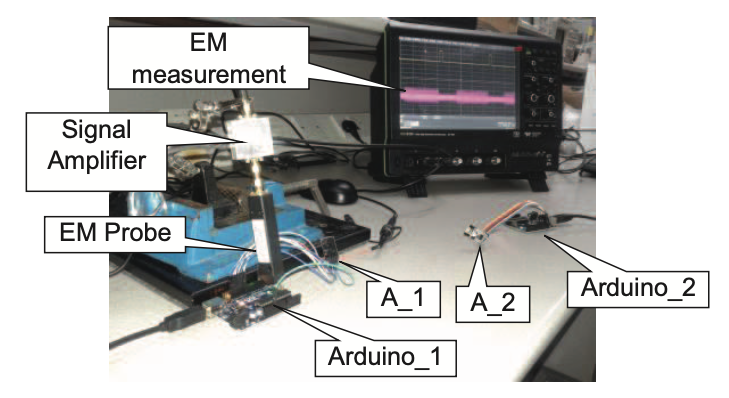
\includegraphics[width=10cm, height=4cm]{media/em_measurment.png}
            \caption{EM measurement of AES-128 based Arduino implementation}
            \label{fig:em_measurment}
        \end{figure}

    Since these devices have limited computing power and a small GE, the operations they perform, such as multiplications and additions, can be analyzed. In contrast, PCs with high computational capabilities are not as easily analyzed for patterns.
    \end{itemize}



\subsection{Mechanisms and Functionality}

Lightweight cryptography is not a separate branch of cryptography, but rather a subset of cryptographic techniques tailored to specific requirements.

Cryptography is generally divided into symmetric cryptography and asymmetric cryptography. In symmetric cryptography, the sender and receiver share the same key. It is considered a fast and secure way of encryption. The main challenge is securely exchanging the key with the communication partner. Furthermore, if the key is revealed, the encryption is compromised. 

In asymmetric encryption, each partner has one private key and one public key. The private key is known only to the owner, while the public key is revealed to the public. The private key is used to decrypt text that has been encrypted with the public key. This way, each partner can use the public key of the other to encrypt text that is meant for the other, and their own private key to decrypt text that is meant for themselves~\cite{ekwueme2024lightweight}. 

Although asymmetric cryptography is secure and solves the problem of key exchange, the keys have to be much longer than in symmetric cryptography. Thus, it is more demanding in terms of hardware resources. Since symmetric cryptography has lower demands in terms of storage, processing power, complexity, and bandwidth, it is considered the preferred method in IoT~\cite{khudoykulov2022comparison}~\cite{ekwueme2024lightweight}.

\begin{figure}[h]
    \centering
    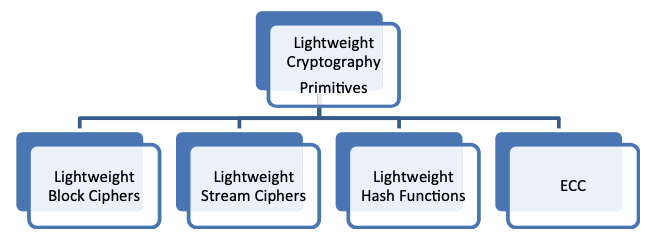
\includegraphics[width=11cm, height=4cm]{media/primitives_for_IoT.png}
    \caption{Lightweight cryptographic primitives for IoT}
    \label{fig:primitives_for_IoT}
\end{figure}


\subsubsection{Classification and Design of Lightweight Primitives}
Similar to conventional cryptography, lightweight cryptography includes four types of primitives: Lightweight Block Ciphers (LWBC), Lightweight Stream Ciphers (LWSC), Lightweight Hash Functions (LWHF), and Elliptic Curve Cryptography (ECC) (Figure~\ref{fig:primitives_for_IoT})~\cite{dhanda2020lightweight}. While stream ciphers have their uses in cryptography for IoT applications, the adaptability of block ciphers is preferred. The similarity between encryption and decryption operations in block ciphers allows for reduced resource consumption and simpler hardware and software implementations.

\textbf{Basic Block Cipher Design}
\begin{itemize}
    \item \textbf{Substitution-box (S-box)}: The S-box performs a substitution operation by taking a small block of input bits (often 4 bits) and transforming them into an output block of bits of the same size. This process, also known as confusion, introduces complexity and unpredictability between input and output bits.
    \item \textbf{Permutation-box (P-box)}: The P-box scatters the output bits of the S-box across the plaintext, ensuring that each change to an input bit influences many output bits. This step, known as diffusion, together with the S-box, makes it harder for an attacker with access to the plaintext and ciphertext to extract the key.
    \item \textbf{Rounds}: In block ciphers, the encryption and decryption processes are divided into several phases called ``rounds''.
    \item \textbf{Substitution-Permutation Network (SPN)}: This is a structure used in each round of encryption, where S-boxes and P-boxes are applied systematically. AES is probably the most popular SPN-based algorithm, with others including PRESENT and GIFT~.
    \item \textbf{The Feistel Network (FN)}: Another structure used in block ciphers is the Feistel Network, where the input block is divided into two equal parts, and during each round, only one half of the block is processed (using substitution and permutation), and then the output is combined with the other half. Some algorithms based on FN include TEA and Camellia~\cite{ekwueme2024lightweight}~\cite{chauhan2022analysis}.
\end{itemize}



\subsection{Unaddressed Needs and Introduction to Ascon}

Just in the last 10 years, Lightweight Cryptography (LWC) has gained attention from the community, thus many aspects were unaddressed in the past. Some of the research gaps for LWC primitives back in 2020 can be seen in Figure~\ref{fig:Research_gaps}~\cite{dhanda2020lightweight}.

\begin{figure}[h]
    \centering
    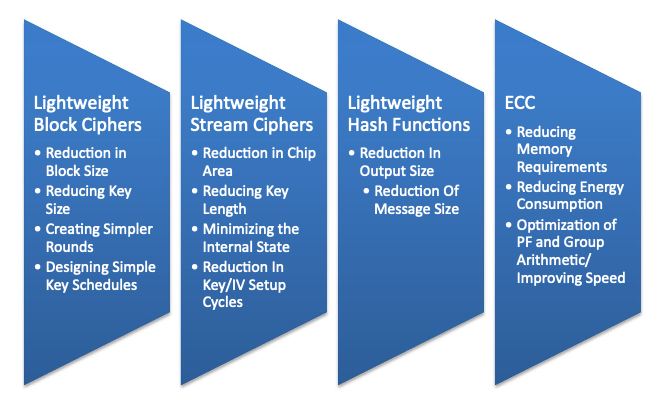
\includegraphics[width=12cm, height=7.5cm]{media/Research_gaps.png}
    \caption{Research gaps for LWC primitives}
    \label{fig:Research_gaps}
\end{figure}

NIST sets rules for Lightweight Cryptography (LWC) to improve performance and security by making specific design decisions, including:

\begin{itemize}
    \item \textbf{Smaller block sizes}: This is done to save memory, but could make the algorithms susceptible to plaintext or key recovery attacks.
    \item \textbf{Smaller key sizes}: In the past, many algorithms used keys less than 96 bits. NIST now requires at least 112 bits.
    \item \textbf{Simpler rounds}: Uses basic components to save space. For example, a 4-bit S-box in PRESENT uses only 28 GEs compared to 395 GEs for the AES S-box. Simpler designs may require more rounds to be secure.
    \item \textbf{Simpler key schedules}: Reduces memory and power needs but may increase vulnerability to certain types of attacks. Secure key functions can help prevent these.
    \item \textbf{Minimal implementations}: Only includes essential functions, which saves space and power. Some devices might only need to encrypt or decrypt, not both~\cite{mckay2016report}.
\end{itemize}

Following the evaluation of the finalists using the specified criteria, NIST has chosen the ASCON family for standardization. This group includes AEAD and hash functions, as well as extra XOFs. The design of ASCON, which is based on permutations, allows it to meet a broad range of application requirements at a low additional cost for implementing new functionalities. A detailed examination of ASCON will be the content of the following chapters~\cite{turan2021status}.


